\section{Phần mở rộng trên Burp Suite}
Như đã giới thiệu ở \textbf{Chương 4}, Burp Suite là một khung thức kiểm thử thâm nhập ứng dụng web được viết trên nền Java. Nó không chỉ nổi tiếng và hữu dụng ở những tính năng cơ bản sẵn có như proxy trung gian, bộ lặp lại (repeater) và tuần tự hóa (sequencer) các request, mà còn ở các phần mở rộng của nó. Burp Suite cho phép và hỗ trợ người dùng tự viết các phần mở rộng (extender) bằng ngôn ngữ Java, Python hoặc Ruby để tiện lợi hóa quá trình sử dụng công cụ này cũng như để phát triển thêm các tính năng có sẵn theo mục đích người dùng. Các phần mở rộng này có thể được công khai trên \textbf{BApp Store} của Burp Suite và được sử dụng như một công cụ độc lập trên nền các tính năng cơ bản của nó. Trong phạm vi luận văn này, chúng tôi sử dụng tính năng proxy trung gian, thâm nhập (intruder) để tạo ra request mẫu và hiện thực một phần mở rộng để gửi \acrshort{http} request mẫu đó đến công cụ \textbf{webfuzzer}.\par
Các đối tượng kiểm thử (\acrshort{http} request mẫu) sẽ được người dùng chọn thông qua trình duyệt web có cài đặt proxy. Bằng việc cài đặt tùy chọn proxy trên trình duyệt và trên Burp Suite về cùng một giá trị IP:port (mặc định là \texttt{127.0.0.1:8080} trên Burp Suite), phần mềm này sẽ bắt được tất cả những request được gửi đi từ phía trình duyệt web người dùng, sau đó cho phép chuyển tiếp (forward), loại bỏ (drop) hoặc chuyển những request mà người dùng muốn kiểm thử đến các mô-đun khác của Burp Suite. Giao diện của mô-đun \textbf{Proxy} trong quá trình bắt request được thể hiện trong Hình \ref{fig:burp-proxy} sau.
\begin{figure}[H]
  \centering
    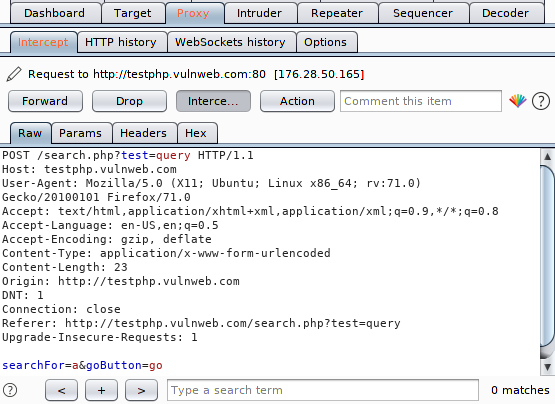
\includegraphics[width=0.75\textwidth,keepaspectratio=true]{images/burp-proxy.png}
  \caption{Sử dụng mô-đun Proxy của Burp Suite để bắt HTTP request}
  \label{fig:burp-proxy}
\end{figure}
Việc tạo request mẫu để gửi cho \textbf{webfuzzer} tiếp tục bằng bước chuyển tiếp request từ \textbf{Proxy} đến mô-đun \textbf{Intruder} để chọn tiếp tham số cần kiểm thử. Mô-đun \textbf{Intruder} chuyên dùng để đánh dấu các vị trí sẽ được thay thế bằng payload bằng cách thêm hoặc bỏ các kí tự ``\texttt{\$}'' bao quanh giá trị của tham số, sau đó chọn chiến lược tấn công (sniper, cluster bomb,...) để gửi đến ứng dụng web mục tiêu. Chúng tôi tận dụng hai mô-đun \textbf{Proxy} và \textbf{Intruder} này để chọn ra đối tượng kiểm thử cho \textbf{webfuzzer}, bao gồm mẫu các tiêu đề \acrshort{http}, đích đến và các tham số cần kiểm thử như Hình \ref{fig:burp-intruder} dưới đây.
\begin{figure}[H]
  \centering
    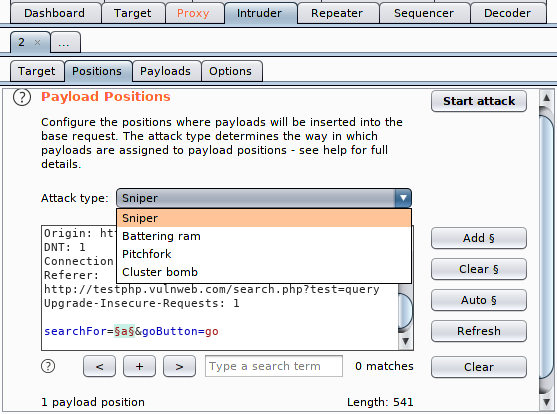
\includegraphics[width=0.75\textwidth,keepaspectratio=true]{images/burp-intruder.png}
  \caption{Giao diện mô-đun Intruder của Burp Suite}
  \label{fig:burp-intruder}
\end{figure}
Sau cùng, chúng tôi hiện thực một phần mở rộng trên Burp Suite để gửi request mẫu đã tạo ra đến công cụ \textbf{webfuzzer}. Burp Suite cung cấp sẵn định dạng các interface cũng như tài liệu Javadoc cần thiết để hiện thực một phần mở rộng như Hình \ref{fig:burp-extender} bên dưới.
\begin{figure}[H]
  \centering
    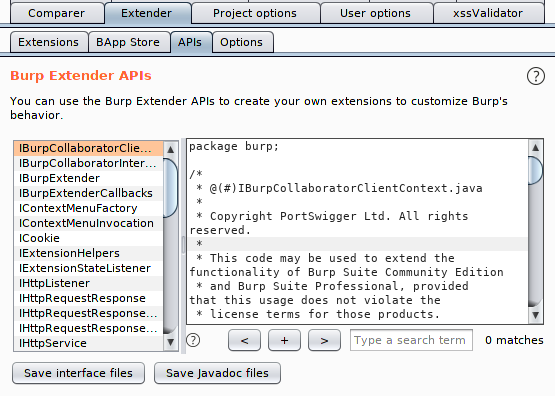
\includegraphics[width=0.75\textwidth,keepaspectratio=true]{images/burp-extender.png}
  \caption{Các phương thức cần để hiện thực một phần mở rộng trên Burp Suite}
  \label{fig:burp-extender}
\end{figure}
Cụ thể, chúng tôi tiến hành xây dựng class \texttt{BurpExtender} bằng cách hiện thực interface \texttt{IBurpExtender} có sẵn, sử dụng ngôn ngữ Java. \textbf{Về giao diện}, phần mở rộng gồm 3 tab chính là ``Configuration'' (chứa textbox nhập địa chỉ IP và port để gửi đến \textbf{webfuzzer}), ``Todo'' và ``About'' dưới dạng các Swing panel trong ngôn ngữ Java. Chúng tôi override lại hàm \texttt{run} của phương thức \texttt{registerExtenderCallbacks} để hiện thực giao diện này.\\
\begin{lstlisting}[language=Java]
@Override
public void run() {
    JPanel jPanel = new JPanel();
    jPanel.setLayout(null);
    JLabel jLabel = new JLabel("Server Address:");
    jLabel.setBounds(10, 10, 500, 30);
    BurpExtender.this.tfServerAdress = new JTextField(BurpExtender.SERVERADRESS);
    BurpExtender.this.tfServerAdress.setBounds(500, 10, 300, 30);
    jPanel.add(jLabel);
    jPanel.add(BurpExtender.this.tfServerAdress);
    JPanel jPanel2 = new JPanel(new GridLayout(2, 1));
    JPanel jPanel3 = new JPanel();
    JLabel jLabel2 = new JLabel("<html><h1>y4t0g4m1 webfuzzer</h1><p>@Author: y4t0g4m1</p><p>@Features:</p></html>");
    jPanel3.add((Component)jLabel2, "Center");
    BurpExtender.this.tabs = new JTabbedPane();
    BurpExtender.this.tabs.add("Configuration", jPanel);
    BurpExtender.this.tabs.add("Todo", jPanel2);
    BurpExtender.this.tabs.add("About", jPanel3);
    BurpExtender.this.mainPanel = new JPanel(new GridLayout(1, 1));
    BurpExtender.this.mainPanel.add(BurpExtender.this.tabs);
    BurpExtender.this.callbacks.customizeUiComponent(
        (Component)BurpExtender.this.tabs);
    BurpExtender.this.callbacks.customizeUiComponent(
        (Component)BurpExtender.this.mainPanel);
    BurpExtender.this.callbacks.addSuiteTab((ITab)BurpExtender.this);
}
\end{lstlisting}
\textbf{Về chức năng}, phần mở rộng này nhận dữ liệu đầu vào là thông tin địa chỉ IP và port của máy chủ công cụ \textbf{webfuzzer}, và nội dung của request mẫu từ mô đun \textbf{Intruder} được hệ thống lại dưới định dạng JSON như sau.\\
\begin{lstlisting}[language=json,firstnumber=1]
"burp":{ 
    "request":"UE9TVCAvc2VhcmNoLnBocD90Z...VhcmNoRm9yPadhpyZnb0J1dHRvbj1nbw==",
    "content_type":"CONTENT_TYPE_URL_ENCODED",
    "body_offset":"516",
    "method":"POST",
    "url":"http://testphp.vulnweb.com:80/search.php?test=query",
    "headers":{ 
        "User-Agent":"Mozilla/5.0 (X11; Ubuntu; Linux x86_64; rv:71.0) Gecko/20100101 Firefox/71.0",
        "Accept":"text/html,application/xhtml+xml,application/xml;q=0.9,*/*;q=0.8",
        "Accept-Language":"en-US,en;q=0.5",
        "Accept-Encoding":"gzip, deflate",
        "Content-Type":"application/x-www-form-urlencoded",
        "Origin":"http://testphp.vulnweb.com",
        "DNT":"1",
        "Connection":"close",
        "Referer":"http://testphp.vulnweb.com/search.php?test=query",
        "Upgrade-Insecure-Requests":"1"
    }
}
\end{lstlisting}
Trường \texttt{request} chứa toàn bộ nội dung của request mẫu dưới dạng base64, các trường còn lại được trích xuất ra bằng các phương thức \texttt{getMethod()}, \texttt{getUrl()}, \texttt{getBodyOffset()}, \texttt{getContentType()}, \texttt{getHeaders()} của class \texttt{IRequestInfo}. Sau đó phần mở rộng tiến hành trích xuất phần thân (body) của request dựa vào giá trị \texttt{body\_offset} thành trường \texttt{data} chứa từng cặp tên tham số - giá trị tương ứng của request. Tiếp theo, nó xây dựng một \acrshort{http} request để gửi request mẫu này tới \textbf{webfuzzer} dưới dạng chuỗi có định dạng JSON được chứa trong phần body của request bằng phương thức \texttt{makeRequest} sau. Địa chỉ IP và port của công cụ được lấy từ textbox ở giao diện và lưu trong biến \texttt{uRL} của class \texttt{BurpExtender} đang hiện thực.\\
\begin{lstlisting}[language=Java]
public IHttpRequestResponse makeRequest(URL uRL, String string) {
    try {
        ArrayList<String> arrayList = new ArrayList<String>();
        arrayList.add("POST / HTTP/1.1");
        arrayList.add("Host: " + uRL.getHost() + ":" + uRL.getPort());
        arrayList.add("User-Agent: BURP18/xnnx");
        arrayList.add("Content-Type: application/json");
        arrayList.add("Connection: close");
        byte[] arrby = this.helpers.stringToBytes(string);
        byte[] arrby2 = this.helpers.buildHttpMessage(arrayList, arrby);
        IHttpRequestResponse iHttpRequestResponse = this.callbacks.makeHttpRequest(this.helpers.buildHttpService(
            uRL.getHost(), uRL.getPort(), uRL.getProtocol() == "https"), arrby2);
        return iHttpRequestResponse;
    }
    catch (Exception exception) {
        this.stdout.println("[!] Loi khi build request toi server: " + exception.getMessage());
        return null;
    }
}
\end{lstlisting}
Kết quả hiện thực của phần mở rộng này là cho phép gửi \acrshort{http} request mẫu từ mô-đun \textbf{Intruder} đến công cụ \textbf{webfuzzer} đã được format lại theo định dạng JSON dưới đây.\\
\begin{lstlisting}[language=json,firstnumber=1]
"python":{ 
    "url":"http://testphp.vulnweb.com:80/search.php?test=query",
    "cookies":"",
    "headers":{ 
        "User-Agent":"Mozilla/5.0 (X11; Ubuntu; Linux x86_64; rv:71.0) Gecko/20100101 Firefox/71.0",
        "Accept":"text/html,application/xhtml+xml,application/xml;q=0.9,*/*;q=0.8",
        "Accept-Language":"en-US,en;q=0.5",
        "Accept-Encoding":"gzip, deflate",
        "Content-Type":"application/x-www-form-urlencoded",
        "Origin":"http://testphp.vulnweb.com",
        "DNT":"1",
        "Connection":"close",
        "Referer":"http://testphp.vulnweb.com/search.php?test=query",
        "Upgrade-Insecure-Requests":"1"
    },
    "data":{ 
        "searchFor":"\xa7a\xa7",
        "goButton":"go"
    },
    "method":"post"
}
\end{lstlisting}
Định dạng JSON trên cũng là cấu trúc thống nhất của một request mẫu trong suốt quá trình kiểm thử và lưu lại nhật kí hoạt động của \textbf{webfuzzer}. Định dạng trên đã được thay đổi một vài lần trong quá trình hiện thực công cụ. Ban đầu chúng tôi sử dụng định dạng JSON nguyên bản như dữ liệu đầu vào của phần mở rộng. Việc này dẫn tới một số khó khăn trong việc chuyển đổi qua lại giữa base64 và chuỗi kí tự thường, tính toán vị trí chèn payload dựa vào trong trường hợp có nhiều hơn một vị trí cần chèn payload, đồng thời cũng gặp khó khăn trong việc lưu lại nhật kí hoạt động một cách minh bạch, dễ kiểm tra lại. Vì những lý do đó, chúng tôi quyết định xây dựng lại request mẫu thành một định dạng thống nhất, tiện lợi hơn để công cụ \textbf{webfuzzer} kiểm thử và ghi nhật kí hoạt động cũng như cho người dùng dễ dàng kiểm tra. Chuỗi ``\texttt{\textbackslash xa7}'' trong trường \texttt{data.searchFor} biểu thị kí tự ``\$'' trong request mẫu. Các kí tự này thường nằm ở trường \texttt{data} hoặc \texttt{url} trong đoạn dữ liệu JSON để đánh dấu những vị trí chèn payload để công cụ xử lí. Hiện tại, sử dụng các mô-đun có sẵn của Burp Suite là phương pháp mạnh mẽ, hiệu quả, trực quan, dễ sử dụng và cá nhân hóa nhất hiện nay để chọn ra \acrshort{http} request cần kiểm thử, so với việc sử dụng các khung thức kiểm thử cũ trên thị trường như BeEF hay Metasploit. 

\section{Máy chủ}

\subsection{Mô-đun xây dựng HTTP request}
Mô-đun này nhận vào request mẫu chứa đầy đủ thông tin và các vị trí cần chèn payload từ mô-đun socket listener ở trên. Đầu tiên mô-đun này sẽ tạo ra thêm các request mẫu dựa trên request mẫu nhận được sao cho trong một request chỉ chứ một vị trí chèn payload. Giả sử trường \texttt{data} trong request mẫu có giá trị như sau.\\
\begin{lstlisting}[language=json,firstnumber=1]
"data":{ 
    "searchFor":"\xa7a\xa7",
    "goButton":"\xa7go\xa7"
}
\end{lstlisting}
Lúc này có hai chỗ cần chèn payload vào, đó là giá trị của trường \texttt{searchFor} và \texttt{goButton}. Trước khi tiến hành chèn payload, mô-đun này sẽ tách request mẫu thành hai request mẫu riêng, mỗi request chứa một vị trí chèn payload. Sau đó mới lần lượt chèn các payload cần kiểm thử vào từng request để dựng thành một HTTP request hoàn chỉnh. Chiến lược này tương đương với chiến lược \texttt{sniper} của mô-đun \textbf{Intruder} của Burp Suite. Đoạn mã Python dưới đây hiện thực quá trình chèn payload và thiết kế hàng đợi của mô-đun này.\\
\begin{python}
def prepareRequest(request, _cfg):
    global queue
    global cfg

    queue = Queue()
    cfg = {}

    fileToFuzz = _cfg["fileToFuzz"]
    respNormal = buildNormalRequest(request)
    parseRequest = ParseRequest(request)
    indexFound = parseRequest.getPatternFromRequest()
    requestList = parseRequest.appendPayloadToRequest(indexFound, fileToFuzz)
    queue = list_to_queue(requestList, queue)

    cfg = {"queue": queue, "respNormal": respNormal, "config":_cfg}

    print(yellow + "Start checking for vulnerabilities...." + end)
    threads = [gevent.spawn(preFuzzing, cfg) for i in range(2)] 
    try:
        gevent.joinall(threads)
    except KeyboardInterrupt as e:
        print(e)
        pass
    print(blue + "Done " + _cfg["label"] + " fuzzing" + end)
\end{python}
Ban đầu chúng tôi gặp rất nhiều khó khăn trong việc lần lượt kiểm thử từng payload đối với một lỗ hổng bảo mật. Lý do vì \acrshort{http} là một giao thức không trạng thái (stateless), một HTTP response trả về tương ứng với duy nhất môt HTTP request trước đó gửi đến ứng dụng web. Trong trường hợp chúng tôi muốn hiện thực được công cụ \texttt{webfuzzer}, điều kiện tiên quyết là phải tuần tự hóa được quá trình kiểm thử trên một danh sách các payload. Điều này có nghĩa là sau khi công cụ gửi request chứa payload 1, phải nhận về response tương ứng thành công mới trước khi gửi tiếp request chứa payload 2, nếu không tuân thủ trình tự trên thì công cụ sẽ không xác định được payload nào gây ra lỗi để ghi lại kết quả kiểm thử. Để giải quyết vấn đề trên, chúng tôi đề xuất hiện thực một hàng đợi, lần lượt đẩy vào từng request với cấu hình kiểm thử loại lỗ hổng tương ứng, dequeue request hiện tại, gửi đi và nhận về response xong mới dequeue request tiếp theo để xử lí. Cấu hình kiểm thử cụ thể sẽ được trình bày ở \textbf{Phần 5.6.1}. Chúng tôi đã sử dụng thư viện \texttt{gevent} của Python để hiện thực hàng đợi này. \texttt{Gevent} là một thư viện gọn nhẹ, hỗ trợ đồng bộ hóa các thao tác giao tiếp với mạng internet nói chung và các ứng dụng web nói riêng dựa trên các trình cộng hành (coroutine-based). Thư viện này cho phép tuần tự hóa quá trình xử lí một hàng đợi các request bằng cách định ra những \textit{đối tượng Greenlet}, các đối tượng này được khai báo kèm theo một hàm thực thi, chỉ khi thực thi xong hàm đó với một đối tượng thì mới được thực thi hàm đó với đối tượng tiếp theo trong hàng đợi. Áp dụng vào công cụ, mỗi request hoàn chỉnh sau khi dựng lên cùng với payload lúc này được đính kèm với hàm \texttt{preFuzzing} và cấu hình tương ứng bằng câu lệnh \\\texttt{threads = [gevent.spawn(preFuzzing, cfg) for i in range(2)]} trong đoạn mã trên. Điều này cho phép mỗi payload cùng với cấu hình tương ứng lần lượt được đưa vào hàm \texttt{preFuzzing} theo thứ tự như chúng tôi mong muốn.

\section{Bộ hậu xử lí và lưu trữ}
Bộ phận này đảm nhiệm việc nhận biết lỗ hổng bảo mật trên ứng dụng web thông qua \acrshort{http} response trả về, đồng thời hiện thực hệ thống quản lý nhật kí hoạt động, ghi lại nhật kí một cách tách bạch, có hệ thống đối với từng request mẫu và từng loại lỗ hổng bảo mật khác nhau.
\subsection{Mô-đun xác nhận lỗi trên HTTP response}
Mô-đun này đảm nhiệm việc xử lí HTTP response trả về từ ứng dụng web và dựa vào response đó để phát hiện lỗ hổng bảo mật. Chúng tôi sử dụng thư viện \texttt{requests} của Python để xử lí \acrshort{http} response trong suốt quá trình tương tác với ứng dụng web mục tiêu. Các response mà mô-đun này nhận được đều thuộc class \texttt{requests.Response}, chúng tôi sử dụng những một số thuộc tính của class này để phục vụ quá trình xử lí kêt quả kiểm thử.
\begin{itemize}
    \item \textbf{status\_code} chứa mã trạng thái của các response trả về.
    \item \textbf{headers} chứa các tiêu đề HTTP của response.
    \item \textbf{text} chứa nội dung unicode của response, có kiểu tùy vào trường \texttt{Content-Type} trên tiêu đề.
    \item \textbf{elapsed} chứa thời gian xử lí request tính theo giây, từ lúc gửi request đến khi nhận được response tương ứng.
\end{itemize}

Kết hợp các cấu hình này và các thuộc tính của biến response trả về, chúng tối định ra chi tiết phương thức phát hiện các lỗ hổng bảo mật như sau.

\subsubsection{Đối với lỗ hổng \acrlong{lfi}}
Để phát hiện lỗ hổng \acrshort{lfi}, chúng tôi thực hiện tương tụ như việc so trùng trong trường hợp \texttt{Content-Type} của response trả về không phải là mã \acrshort{html} đối với lỗ hổng \acrshort{xss}. Cụ thể, chúng tôi cố gắng đọc nội dung tập tin \texttt{/etc/passwd} bằng các payload được chèn vào, tập tin này luôn bắt đầu bằng chuỗi ``\texttt{root:x:}'' trên các máy chủ ứng dụng web nhân Unix. Một khi response trả về có chuỗi này thì khả năng rất cao ứng dụng web mắc phải lỗ hổng \acrshort{lfi}.\par
Tuy nhiên cũng có khả năng các payload này đọc được một tập tin \texttt{/etc/passwd} giả trong quá trình kiểm thử. Ứng dụng web có thể thêm vào thư mục lưu trữ trang web một đường dẫn đến tập tin \texttt{/etc/passwd} có chứa chuỗi ``\texttt{root:x:}'' trong nội dung. Để khắc phục nhược điểm đó, trong tương lai chúng tôi sẽ thiết kế thêm các cấu hình cũng như payload để đọc thêm nhiều tập tin thông tin hệ thống trên Unix khác như \texttt{/etc/issue}, \texttt{/etc/passwd}, \texttt{/etc/shadow}, \texttt{/etc/group}, \texttt{/etc/hosts}, \texttt{/etc/motd}, \texttt{/etc/mysql/my.cnf}, \texttt{/proc/self/environ}, \texttt{/proc/version}, \texttt{/proc/cmdline},... sau khi đã \texttt{[passed]} được tập tin \texttt{/etc/passwd}. Điều này sẽ giúp giảm tỉ lệ dương tính giả của phương pháp phát hiện này. Đồng thời chúng tôi cũng sẽ mở rộng phạm vi phát hiện trên các ứng dụng web chạy trên hệ điều hành Windows Server bằng các payload đọc các tập tin thông tin hệ thống trên Windows như \texttt{boot.ini}, \texttt{windows/win.ini}, \texttt{winnt/win.ini},... Hiện tại do giới hạn thời gian và nguồn lực mà chúng tôi chưa thể triệt tiêu hoàn toàn tỉ lệ dương tính giả trong việc phát hiện lỗ hổng bảo mật này.

\subsubsection{Đối với lỗ hổng time-based \acrlong{sqli}}
Để phát hiện lỗ hổng này, chúng tôi dựa vào thuộc tính \texttt{elapsed} chứa thời gian xử lí request của ứng dụng web và thuộc tính \texttt{time} trong thiết lập cấu hình để loại bỏ những request được xử lí quá nhanh. Các payload kiểm thử lỗ hổng này đều dùng hàm hoãn thời gian 10 giây (\texttt{SLEEP(10), PG\_SLEEP(10), WAITFOR DELAY '0:0:10', WAITFOR TIME '0:0:10'}) kết hợp với việc sử dụng hàm benchmark trả về tổng thời gian thực thi lệnh \texttt{MD5('Y4T0G4M11337')} 1000000 lần cộng với các cách thức đóng ngoặc, chú thích để tránh gặp lỗi cú pháp trong quá trình thực thi câu lệnh SQL chứa payload ở phía máy chủ. Về mặt lý thuyết, nếu ứng dụng web mắc lỗi này thì thời gian xử lí một request chứa các payload kiểm thử không thể ít hơn 10 giây được. Về mặt thực tế, khi kiểm thử một số trang web bằng \textbf{webfuzzer} thì thời gian xử lí các request chứa payload này dao động từ 20 giây đến 60 giây. Đó là lý do chúng tôi đặt thời gian tối đa cho một request kiểm thử là 70 giây, nếu thời gian thực hiện quá 70 giây thì chúng tôi đánh dấu payload tương ứng là \texttt{[skeptical]} vì vẫn có trường hợp thời gian xử lí lâu hơn 60 giây ở các máy chủ web cấu hình thấp hơn. Câu lệnh dưới đây có chức năng tạo, gửi request kèm cài đặt thời gian timed-out là 70 giây và nhận về một giá trị thuộc class \texttt{requests.Response} gán vào biến \texttt{resp}.\\
\begin{python}
resp = request(self.method, self.url, cookies=self.cookies, headers=self.headers, data=self.data, timeout=70)
\end{python}
Đoạn mã Python dưới đây hiện thực quá trình phát hiện lỗ hổng time-based \acrshort{sqli} theo cấu hình và phương pháp đã định trước. Biến \texttt{isTimedOut} có giá trị là \texttt{True} khi đã có ngoại lệ về thời gian xảy ra trong quá trình thực hiện request. Nếu bị timed-out trong lúc kiểm thử lỗ hổng time-based \acrshort{sqli} (\texttt{config['id'] == 3}) thì chúng tôi đánh dấu payload hiện tại là \texttt{[skeptical]}. Còn lại trong trường hợp request được xử lí bình thường thì miễn thời gian trả về response từ ứng dụng web lớn hơn thời gian được thiết lập trong thuộc tính \texttt{time} của cấu hình thì chắc chắn ứng dụng web có lỗ hổng này. Tỉ lệ dương tính giả đối với các trường hợp kiểm thử đã \texttt{[passed]} là bằng 0.\\
\begin{python}
def timebasedDetect(req, resp, payload, isTimedOut, config, method=None):
    if isTimedOut:
        if config['id'] == 3:
            print(purple + "[skeptical]    " + yellow + payload + "\t" + end)
            addToLog(req, config['label'], "SKEPTICAL: " + unescapePayload(payload), method, config["output"])
    else:
        print(red + "[failed]    " + yellow + payload + "\t" +  end)
    elif int(resp.elapsed.total_seconds()) > config['time']:
        print(green + "[passed]    " + yellow + str(resp.status_code) + "\t" + str(len(resp.text)) + "\t" + "{:<10}".format(str(resp.elapsed.total_seconds())) + "\t" +  payload + "\t"+ end)
        addToLog(req, config['label'], unescapePayload(payload), method, config["output"])
    else:
        print(red + "[failed]    " + yellow + str(resp.status_code) + "\t" + str(len(resp.text)) + "\t" + "{:<10}".format(str(resp.elapsed.total_seconds())) + "\t" +  payload + "\t" +  end)
\end{python}
